\documentclass{beamer}
\usepackage{slides}

\newcommand{\rdiv}{\mid_\rightarrow}
\newcommand{\ldiv}{\mid_\leftarrow}
\newcommand{\mat}[1]{\begin{pmatrix} #1 \end{pmatrix}}

\title{Quaternions}
\date{October 2024}

\begin{document}

\frame{\titlepage}

\begin{frame}
	\frametitle{Roadmap}
	\begin{itemize}
		\ii Number theory over ``exotic'' domains to prove two nontrivial theorems (Fermat's Christmas theorem, Lagrange's four-square theorem)
		\ii A first taste of ring theory
	\end{itemize}
\end{frame}

\begin{frame}
	\frametitle{Table of Contents}
	\tableofcontents
\end{frame}

\section{First definitions and history}

\begin{frame}
	\frametitle{First definitions}
	\begin{itemize}
		\ii The complex numbers $\CC$ are made by adding $\sqrt{-1}$ to $\RR$.
		\ii The quaternions $\HH$ are made by adding \emph{three} different $\sqrt{-1}$s to $\RR$.
	\end{itemize}
	
	\begin{definition}
		A quaternion is a number of the form
		\[a = a_1 + a_2i + a_3j + a_4k\]
		for reals $a_1,a_2,a_3,a_4$ and the ``square roots of $-1$'' $i$, $j$, and $k$. Addition is done in the obvious way. Multiplication is distributive over addition and associative, and
		\[i^2 = j^2 = k^2 = -1 \qquad ij = -ji = k \qquad jk = -kj = i \qquad ki = -ik = j.\]
	\end{definition}
\end{frame}

\begin{frame}
	\frametitle{First definitions}
	\begin{itemize}
		\ii \alert{Multiplication is not in general commutative}, but the real quaternions commute with every element. So $\lambda h = h\lambda$ for all $\lambda \in \RR$ and $h \in \HH$.
		\ii The \emph{conjugate} of $a = a_1 + a_2i + a_3j + a_4k$ is $a^* = a_1 - a_2i - a_3j - a_4k$.
		\ii The \emph{norm} of $a$ is $\abs a = \sqrt{a_1^2 + a_2^2 + a_3^2 + a_4^2} = \sqrt{aa^*} = \sqrt{a^*a}$.
		\ii We have $\abs{ab} = \abs a \abs b$.
		\ii We have $(ab)^* = b^*a^*$. In general, this is not equal to $a^*b^*$.
		\ii The multiplicative inverse of $a$ is $a^{-1} = \frac{a^*}{\abs a^2}$.
		\ii Usually we don't write $\frac ab$, unless one of $a$ or $b$ is real, since multiplication isn't commutative.
	\end{itemize}
\end{frame}

\begin{frame}
	\frametitle{History}
	\emph{Every morning in the early part of October 1843, on my coming down to breakfast, your brother William Edwin and yourself used to ask me: ``Well, Papa, can you multiply triples?'' Whereto I was always obliged to reply, with a sad shake of the head, ``No, I can only add and subtract them.''}

	\medskip

	---A letter from Hamilton to his son Archibald

	\bigskip

	\emph{And here there dawned on me the notion that we must admit, in some sense, a fourth dimension of space for the purpose of calculating with triples\dots{} An electric circuit seemed to close, and a spark flashed forth.}

	\medskip

	---A letter from Hamilton to his friend and colleague John Graves, inventor of the octonions, an eight-dimensional number system
\end{frame}

\begin{frame}
	\frametitle{History}
	\begin{figure}
		\centering
		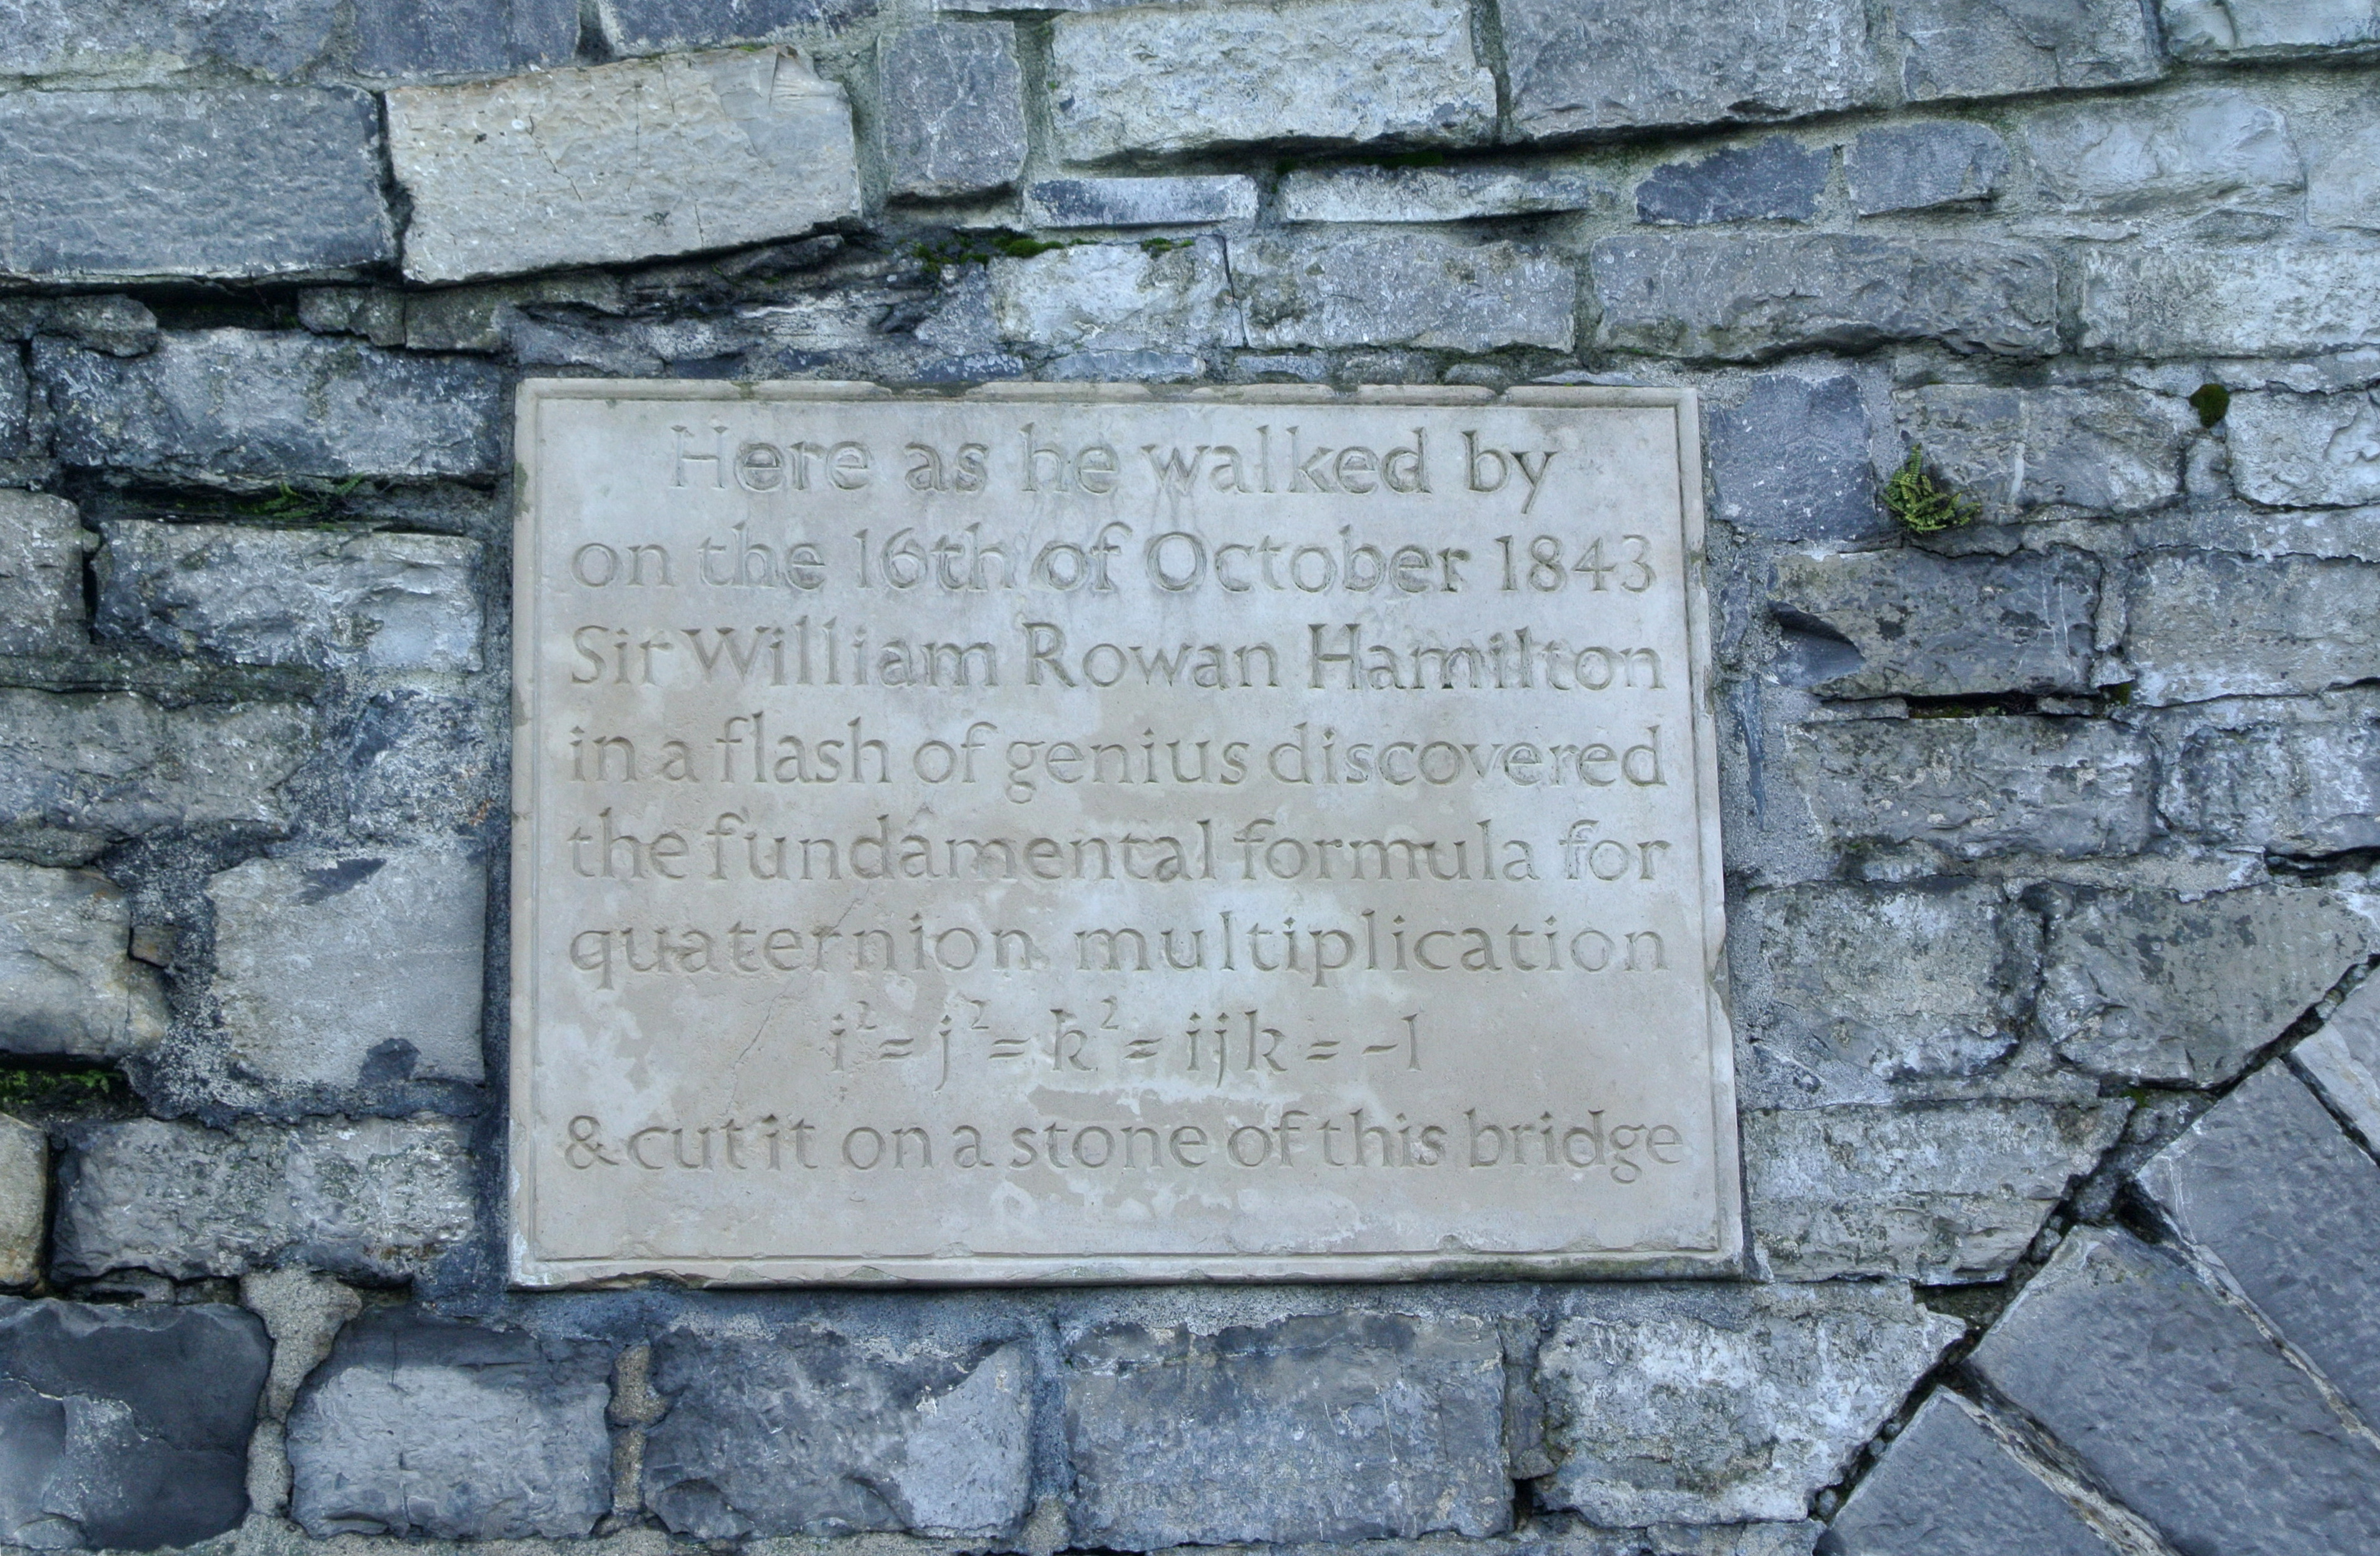
\includegraphics[width=0.8\linewidth]{quaternion_plaque.jpg}
		\caption{A plaque on the Brougham Bridge commemorating the discovery of quaternions. Observe the identity $i^2 = j^2 = k^2 = ijk = -1$.}
	\end{figure}
\end{frame}

\section{\texorpdfstring{Warm-up over $\ZZ$}{}}

\begin{frame}
	\frametitle{Euclid's lemma}
	The goal of this section is to prove the following intuitive lemma.
	\begin{lemma}[Euclid's lemma]
		If $p$ is a prime and $p \mid mn$, then $p \mid m$ or $p \mid n$.
	\end{lemma}
	(Actually, in ring theory, this is how you \emph{define} a prime. Don't worry about that for now. Here a prime number is one that's divisible only by $1$ and itself.)
\end{frame}

\begin{frame}
	\frametitle{Euclidean algorithm setup}
	\begin{itemize}
		\ii For $d,n \in \ZZ$, we say $d$ \emph{divides} $n$, written $d \mid n$, if $n = dk$ for some $k \in \ZZ$.
		\ii For $p \in \ZZ$, we say $p$ is \emph{prime} if $d \mid p$ implies $\abs d = 1$ or $\abs d = p$.
	\end{itemize}

	The following three facts will allow us to perform the Euclidean algorithm.
	
	\begin{block}{}
		If $d \mid m,n$, then $d \mid m - kn$ for $k \in \ZZ$.
	\end{block}
	Let $m = ad$ and $n = bd$, then $m - kn = ad - kbd = (a - kb)d$.

	\begin{block}{}
		For all $x \in \RR$, there is some $k \in \ZZ$ such that $\abs{x - k} < 1$.
	\end{block}
	Easy.
	
	\begin{block}{}
		For all $m,n \in \ZZ$ and $n \neq 0$, there is some $k \in \ZZ$ such that $\abs{m - kn} < \abs n$.
	\end{block}
	Let $x = \frac mn$, there is some $k \in \ZZ$ such that $\abs{\frac mn - k} < 1$. Multiplying by $\abs n$ gives $\abs{m - kn} < \abs n$.
\end{frame}

\begin{frame}
	\frametitle{The Euclidean algorithm}
	\begin{itemize}
		\ii If $d \mid m,n$, then $d \mid m - kn$ for $k \in \ZZ$.
		\ii For all $m,n \in \ZZ$ and $n \neq 0$, there is some $k \in \ZZ$ such that $\abs{m - kn} < \abs n$.
	\end{itemize}

	Let's do the Euclidean algorithm:
	\begin{itemize}
		\ii Start with integers $m$ and $n$ (WLOG $\abs m \ge \abs n$).
		\ii Let $(m_0,n_0) = (m,n)$.
		\ii For $i \ge 1$, let $(m_{i + 1},n_{i + 1}) = (n_i,m_i - k_in_i)$ where $k_i$ is chosen such that $\abs{m_i - k_in_i} < \abs n$.
		\ii Let $\gcd(m,n)$ be the value of $m_i$ when $n_i$ first reaches $0$.
		\ii There are integers $a$ and $b$ such that $\gcd(m,n) = am + bn$.
	\end{itemize}
\end{frame}

\begin{frame}
	\frametitle{A concrete example}
	Example with $(m,n) = (30,21)$:
	\begin{align*}
		(m_0,n_0) &= (30,21) = (m,n) \\
		(m_1,n_1) &= (21,9) = (n,m - n) \\
		(m_2,n_2) &= (9,3) = (m - n,-2m + 3n) \\
		(m_3,n_3) &= (3,0) = (-2m + 3n,7m - 10n).
	\end{align*}

	Note that:
	\begin{itemize}
		\ii At each step, $m_i$ and $n_i$ are linear combinations of $m$ and $n$.
		\ii In particular, $\gcd(m,n) = m_3 = 3$ is a linear combination of $m$ and $n$. That is, for any $m$ and $n$, there exist integers $a$ and $b$ such that $am + bn = \gcd(m,n)$. This is known as B\'ezout's identity.
		\ii Also, $\gcd(m,n)$ divides each $m_i$ and $n_i$.
	\end{itemize}
	
	Try the cases $(m,n) = (24,20)$ and $(m,n) = (42,-30)$.
\end{frame}

\begin{frame}
	\frametitle{Euclid's lemma}
	\begin{lemma}[Euclid's lemma]
		If $p$ is a prime and $p \mid mn$, then $p \mid m$ or $p \mid n$.
	\end{lemma}
	
	\begin{proof}
		Suppose $p \mid mn$ and $p \nmid m$. Then $\abs{\gcd(p,m)} = 1$, so by B\'ezout's identity there are integers $a$ and $b$ such that $ap + bm = 1$. So $apn + bmn = n$, but since $p \mid apn + bmn$, $p \mid n$.
	\end{proof}

	Now let's do the same thing over the Gaussian integers!
\end{frame}

\section{The Gaussian integers and Fermat's Christmas theorem}

\begin{frame}
	\frametitle{Some definitions}
	The Gaussian integers are the set
	\[\ZZ[i] = \{a + bi \mid a,b \in \ZZ\} \subseteq \CC.\]

	Observe that
	\begin{itemize}
		\ii For all $n \in \ZZ[i]$, $\abs n^2$ is an integer.
		\ii The Gaussian integers are closed under addition and multiplication.
	\end{itemize}

	We set up the exact same definitions:
	\begin{itemize}
		\ii For $d,n \in \ZZ[i]$, we say $d$ \emph{divides} $n$, written $d \mid n$, if $n = dk$ for $k \in \ZZ[i]$.
		\ii For $p \in \ZZ[i]$, we say $p$ is \emph{prime} if $d \mid p$ implies $\abs d = 1$ or $\abs d = \abs p$.
	\end{itemize}

	We will prove Euclid's lemma again:
	\begin{lemma}[Euclid's lemma]
		Let $p,m,n \in \ZZ[i]$ with $p$ prime. If $p \mid mn$, then $p \mid m$ or $p \mid n$.
	\end{lemma}
\end{frame}

\begin{frame}
	\frametitle{The same three claims}
	\begin{block}{}
		If $d \mid m,n$, then $d \mid m - kn$ for $k \in \ZZ[i]$.
	\end{block}
	Let $m = ad$ and $n = bd$, then $m - kn = ad - kbd = (a - kb)d$.

	\begin{block}{}
		For all $x \in \CC$, there is some $k \in \ZZ[i]$ such that $\abs{x - k} < 1$.
	\end{block}
	Let $x = x_1 + x_2i$ and $k = k_1 + k_2i$, we may force $\abs{x_1 - k_1} \le \frac12$ and $\abs{x_2 - k_2} \le \frac12$, then $\abs{x - k} = \sqrt{(x_1 - k_1)^2 + (x_2 - k_2)^2} \le \frac{\sqrt 2}2 < 1$.
	
	\begin{block}{}
		For all $m,n \in \ZZ[i]$ and $n \neq 0$, there is some $k \in \ZZ[i]$ such that $\abs{m - kn} < \abs n$.
	\end{block}
	Let $x = \frac mn$, there is some $k \in \ZZ[i]$ such that $\abs{\frac mn - k} < 1$. Multiplying by $\abs n$ gives $\abs{m - kn} < \abs n$.
\end{frame}

\begin{frame}
	\frametitle{The same Euclidean algorithm}
	\begin{itemize}
		\ii Start with $m,n \in \ZZ[i]$ (WLOG $\abs m \ge \abs n$).
		\ii Let $(m_0,n_0) = (m,n)$.
		\ii For $i \ge 1$, let $(m_{i + 1},n_{i + 1}) = (n_i,m_i - k_in_i)$ where $k_i$ is chosen such that $\abs{m_i - k_in_i} < \abs n$.
		\ii Let $\gcd(m,n)$ be the value of $m_i$ when $n_i$ first reaches $0$.
		\ii There are $a,b \in \ZZ[i]$ such that $\gcd(m,n) = am + bn$.
	\end{itemize}
\end{frame}

\begin{frame}
	\frametitle{A concrete example}
	Example with $(m,n) = (-6 + 7i,3 + 4i)$:
	\begin{align*}
		(m_0,n_0) &= (-6 + 7i,3 + 4i) = (m,n) \\
		(m_1,n_1) &= (3 + 4i,-6 + 7i - 2i(3 + 4i)) \\
		&= (3 + 4i,2 + i) = (n,m - 2in) \\
		(m_2,n_2) &= (2 + i,3 + 4i - (2 + i)(2 + i)) \\
		&= (2 + i,0) = (m - 2in,(-2 - i)m + (-1 + 4i)n)
	\end{align*}

	Again, note that:
	\begin{itemize}
		\ii At each step, $m_i$ and $n_i$ are linear combinations of $m$ and $n$.
		\ii In particular, $\gcd(m,n) = m_2 = 2 + i$ is a linear combination of $m$ and $n$.
		\ii Also, $\gcd(m,n)$ divides each $m_i$ and $n_i$.
	\end{itemize}
\end{frame}

\begin{frame}
	\frametitle{Euclid lemma 2: electric boogaloo}
	\begin{lemma}[Euclid's lemma]
		Let $p,m,n \in \ZZ[i]$ with $p$ prime. If $p \mid mn$, then $p \mid m$ or $p \mid n$.
	\end{lemma}
	
	\begin{proof}
		Suppose $p \mid mn$ and $p \nmid m$. Then $\abs{\gcd(p,m)} = 1$, so by B\'ezout's identity there are Gaussian integers $a$ and $b$ such that $ap + bm = \gcd(p,m)$, or equivalently, multiplying by $\overline{\gcd(p,m)}$, there are Gaussian integers $a'$ and $b'$ such that $a'p + b'm = 1$. So $apn + bmn = n$, but since $p \mid apn + bmn$, $p \mid n$.
	\end{proof}
\end{frame}

\begin{frame}
	\frametitle{Fermat's Christmas theorem}
	This is enough to extract the following:

	\begin{theorem}[Fermat's Christmas theorem]
		Let $p \in \ZZ$ be a prime. Then $p = x^2 + y^2$ for some $x,y \in \ZZ$ iff $p = 2$ or $p \equiv 1 \pmod 4$.
	\end{theorem}

	Note that $2 = 1^2 + 1^2$ and $3 \pmod 4$ primes fail modulo $4$. So we just need to show each $1 \pmod 4$ prime is the sum of two squares.

	\begin{lemma}
		If $p \equiv 1 \pmod 4$, then $p \mid 1 + a^2$ for some $a \in \ZZ$.
	\end{lemma}

	\begin{itemize}
		\ii Write $p = 4k + 1$ and consider the polynomial $x^{4k} - 1 = (x^{2k} - 1)(x^{2k} + 1)$ modulo $p$.
		\ii This has $p - 1 = 4k$ roots modulo $p$ by FLT, so $x^{2k} - 1$ and $x^{2k} + 1$ each have exactly $2k$ roots by counting degrees.
		\ii So $x^{2k} + 1$ has some root modulo $p$, so $p \mid (x^k)^2 + 1$, done.
	\end{itemize}
\end{frame}

\begin{frame}
	\frametitle{Fermat's Christmas theorem}
	\begin{lemma}
		Any $1 \pmod 4$ prime $p$ is \alert{not} prime in the Gaussian integers.
	\end{lemma}

	\begin{itemize}
		\ii If $p$ was prime, $p \mid 1 + a^2 = (1 + ai)(1 - ai)$ for some $a \in \ZZ$, so $p \mid 1 + ai$ or $p \mid 1 - ai$ by Euclid's lemma.
		\ii But neither $\frac1p + \frac api$ nor $\frac1p - \frac api$ are Gaussian integers, done.
	\end{itemize}

	\medskip

	Now here's the main proof:

	\begin{itemize}
		\ii Since $p$ is not irreducible in $\ZZ[i]$, write $p = mn$ with $\abs m,\abs n \neq 1,\abs p$.
		\ii Squaring and taking the norm, $\abs m^2\abs n^2 = p^2$, but since $\abs m^2,\abs n^2 \in \ZZ$, $\abs m^2 = \abs n^2 = p$.
		\ii If $m = x + yi$, then $\abs m^2 = x^2 + y^2 = p$, as desired.
	\end{itemize}
	Now let's do the same thing over the Hurwitz integers!
\end{frame}

\section{Hurwitz quaternions and the four-square theorem}

\begin{frame}
	\frametitle{The Hurwitz integers}
	\begin{definition}
		The Hurwitz quaternions $H$ are the set of quaternions whose coefficients are either all integers or all half-integers. In particular, Hurwitz integers cannot have a mix of integer and half-integer coefficients.
	\end{definition}
	
	Observe that
	\begin{itemize}
		\ii For all $h \in H$, $\abs h^2$ is an integer.
		\ii The Hurwitz integers are closed under addition and multiplication.
	\end{itemize}
\end{frame}

\begin{frame}
	\frametitle{The same definitions}
	\begin{itemize}
		\ii For $h,n \in H$, we say $d$ \emph{right divides} $h$, written $d \rdiv h$, if $h = ad$ for some $a \in H$. We say $d$ \emph{left divides} $h$, written $d \ldiv h$, if $h = db$ for some $b \in H$.\footnote{I just made up the notation $\rdiv$ and $\ldiv$ for right and left divisibility. I'm not sure if any standard notation exists.}
		\ii A Hurwitz integer $p$ is called \emph{prime} if $d \rdiv p$ implies $\abs d = 1$ or $d = \abs p$.
	\end{itemize}

	We require two notions of divisibility because multiplication is not commutative.

	We will prove the following. Looks familiar?

	\begin{lemma}[Weak Euclid's lemma]
		Let $p \in H$ be a real Hurwitz prime. Then if $p \mid mn$, $p \mid m$ or $p \mid n$.
	\end{lemma}
\end{frame}

\begin{frame}
	\frametitle{The same three claims, again}
	\begin{block}{}
		If $d \rdiv m,n$, then $d \rdiv m - hn$ for $h \in H$.
	\end{block}
	Let $m = ad$ and $n = bd$, then $m - hn = ad - hbd = (a - hb)d$.

	\begin{block}{}
		For all $x \in \HH$, there is some $h \in H$ such that $\abs{x - k} < 1$.
	\end{block}
	Write $x = x_1 + x_2i + x_3j + x_4k$ and $h = h_1 + h_2i + h_3j + h_4k$. We may force $\abs{x_1 - h_1} \le \frac14$ and $\abs{x_i - h_i} \le \frac12$ for $i = 2,3,4$. Then $\abs{x - h} = \sqrt{(x_1 - h_1)^2 + \sum_{i = 2}^4(x_i - h_i)^2} \le \sqrt{\left(\frac14\right)^2 + 3\left(\frac12\right)^2} < 1$, as desired.
	
	\begin{block}{}
		For all $m,n \in H$ and $n \neq 0$, there is some $h \in H$ such that $\abs{m - hn} < \abs n$.
	\end{block}
	Let $x = mn^{-1}$, then there is some $h \in H$ such that $\abs{mn^{-1} - h} < 1$. Right multiplying by $\abs n$, $\abs{m - hn} < \abs n$, as desired.
\end{frame}

\begin{frame}
	\frametitle{The Euclidean algorithm, again}
	\begin{itemize}
		\ii Start with $m,n \in H$ (WLOG $\abs m \ge \abs n$).
		\ii Let $(m_0,n_0) = (m,n)$.
		\ii For $i \ge 1$, let $(m_{i + 1},n_{i + 1}) = (n_i,m_i - k_in_i)$ where $k_i$ is chosen such that $\abs{m_i - k_in_i} < \abs n$.
		\ii Let $\gcd(m,n)$ be the value of $m_i$ when $n_i$ first reaches $0$.
		\ii There are $a,b \in H$ such that $\gcd(m,n) = am + bn$.
	\end{itemize}
\end{frame}

\begin{frame}
	\frametitle{Weak Euclid's lemma}
	\begin{lemma}[Weak Euclid's lemma]
		Let $p \in H$ be a real Hurwitz prime. Then if $p \mid mn$, $p \mid m$ or $p \mid n$.
	\end{lemma}

	\begin{proof}
		Suppose $p \mid mn$ and $p \nmid m$. Then $\abs{\gcd(p,m)} = 1$, so by B\'ezout's identity there are Hurwitz integers $a$ and $b$ such that $ap + bm = \gcd(p,m)$, or equivalently, left multiplying by $\gcd(p,m)^*$, there are Hurwitz integers $a'$ and $b'$ such that $a'p + b'm = 1$. So $apn + bmn = n$, but since $p \mid apn + bmn$, $p \mid n$.
	\end{proof}
\end{frame}

\begin{frame}
	\frametitle{Lagrange's four-square theorem}
	Now this is enough to extract the following.

	\begin{theorem}[Lagrange's four-square theorem]
		Every positive integer is the sum of four squares.
	\end{theorem}

	\begin{itemize}
		\ii Observe that $1$ works.
		\ii We must show that for every positive integer $a$, there is some quaternion with integer coefficients $m$ such that $\abs m^2 = a$.
		\ii Since $\abs{mn} = \abs m\abs n$, it's enough to show the result for all primes.
		\ii Actually, since $\abs{1 + i} = \sqrt 2$, it's enough to show the result for all odd primes.
	\end{itemize}
\end{frame}

\begin{frame}
	\frametitle{Lagrange's four-square theorem}
	\begin{lemma}
		For odd primes $p$, $p \mid 1 + a^2 + b^2$ for some integers $a$ and $b$.
	\end{lemma}

	\begin{itemize}
		\ii There are $\frac{p + 1}2$ perfect squares modulo $p$.
		\ii So there are $\frac{p + 1}2$ elements of the form $-1 - a^2$ modulo $p$.
		\ii So by pigeonhole, since $\frac{p + 1}2 + \frac{p + 1}2 > p$, there must be some perfect square $b^2$ that is of the form $-1 - a^2$ modulo $p$.
		\ii So $-1 - a^2 \equiv b^2 \pmod p$ or $p \mid 1 + a^2 + b^2$.
	\end{itemize}

	\begin{lemma}
		Any odd prime $p$ is \alert{not} prime in the Hurwitz integers.
	\end{lemma}

	\begin{itemize}
		\ii If $p$ was prime, since $p \mid 1 + a^2 + b^2 = (1 + ai + bj)(1 - ai - bj)$ for some $a,b \in \ZZ$, $p \mid 1 + ai + bj$ or $p \mid 1 - ai - bj$ by weak Euclid's lemma.
		\ii But neither $\frac 1p + \frac api + \frac bpj$ nor $\frac 1p - \frac api - \frac bpj$ are Hurwitz integers.
	\end{itemize}
\end{frame}

\begin{frame}
	\frametitle{Lagrange's four-square theorem}
	Here's the main proof:
	\begin{itemize}
		\ii Since $p$ is not irreducible in $H$, write $p = mn$ with $\abs m,\abs n \neq 1,p$.
		\ii Squaring and taking the norm, $\abs m^2\abs n^2 = p^2$, but since $\abs m^2,\abs n^2 \in \ZZ$, $\abs m^2 = \abs n^2 = p$.
		\ii If $m$ has integer coefficients, we are done. Otherwise, pick $\epsilon = \frac12(\pm 1 \pm i \pm j \pm k)$ such that $m' := m + \epsilon$ has even integer coefficients.
		\ii But then $p = mm^* = (m' - \epsilon)(m'^* - \epsilon^*) = (m' - \epsilon)\epsilon^*\epsilon(m^* - \epsilon^*) = (m'\epsilon^* - 1)(\epsilon m'^* - 1)$.
		\ii Since $m'$ has even integer coefficients, $m'\epsilon^* - 1$ and $\epsilon m'^* - 1$ have integer coefficients.
		\ii But $\abs{m'\epsilon^* - 1} = \abs{\epsilon m'^* - 1} = \sqrt p$, which concludes.
	\end{itemize}
\end{frame}

\section{The cross product and the octonions}

\begin{frame}
	\frametitle{The cross product and quaternions}
	Consider the vectors $i,j,k \in \RR^3$ with $i = (1,0,0)$, $j = (0,1,0)$, and $k = (0,0,1)$. The cross product gives
	\begin{align*}
		i \times j &= -j \times i = k \\
		j \times k &= -k \times j = i \\
		k \times i &= -i \times k = j.
	\end{align*}

	Look familiar? Remember the quaternion multiplication identities
	\[ij = -ji = k \qquad jk = -kj = i \qquad ki = -ik = j.\]
\end{frame}

\begin{frame}
	\frametitle{The cross product and quaternions}
	Consider the quaternions with no real part $x = x_1i + x_2j + x_3k$ and $y = y_1i + y_2j + y_3k$. Then if $xy = z_1i + z_2j + z_3k$, then
	\[\mat{x_1 \\ x_2 \\ x_3} \times \mat{y_1 \\ y_2 \\ y_3} = \mat{z_1 \\ z_2 \\ z_3}.\]
	
	Observe that the \emph{right-hand rule} implies there are two ways to define the cross product. Similarly, there are two ways to define quaternion multiplication, one may define $ij = -k$ instead.
\end{frame}

\begin{frame}
	\frametitle{Octonions}
	\emph{If with your alchemy you can make three pounds of gold, why should you stop there?}

	\medskip

	---John T. Graves (inventor of the octonions) in a letter to Hamilton

	\bigskip

	\begin{itemize}
		\ii An \emph{eight}-dimensional number system invented by Graves with \emph{seven} square roots of $-1$
		\ii Not even associative, but alternative: $x(xy) = (xx)y$ and $(yx)x = y(xx)$.
	\end{itemize}
\end{frame}


\begin{frame}
	\frametitle{The octonion multiplication table}
	\begin{figure}
		\centering
		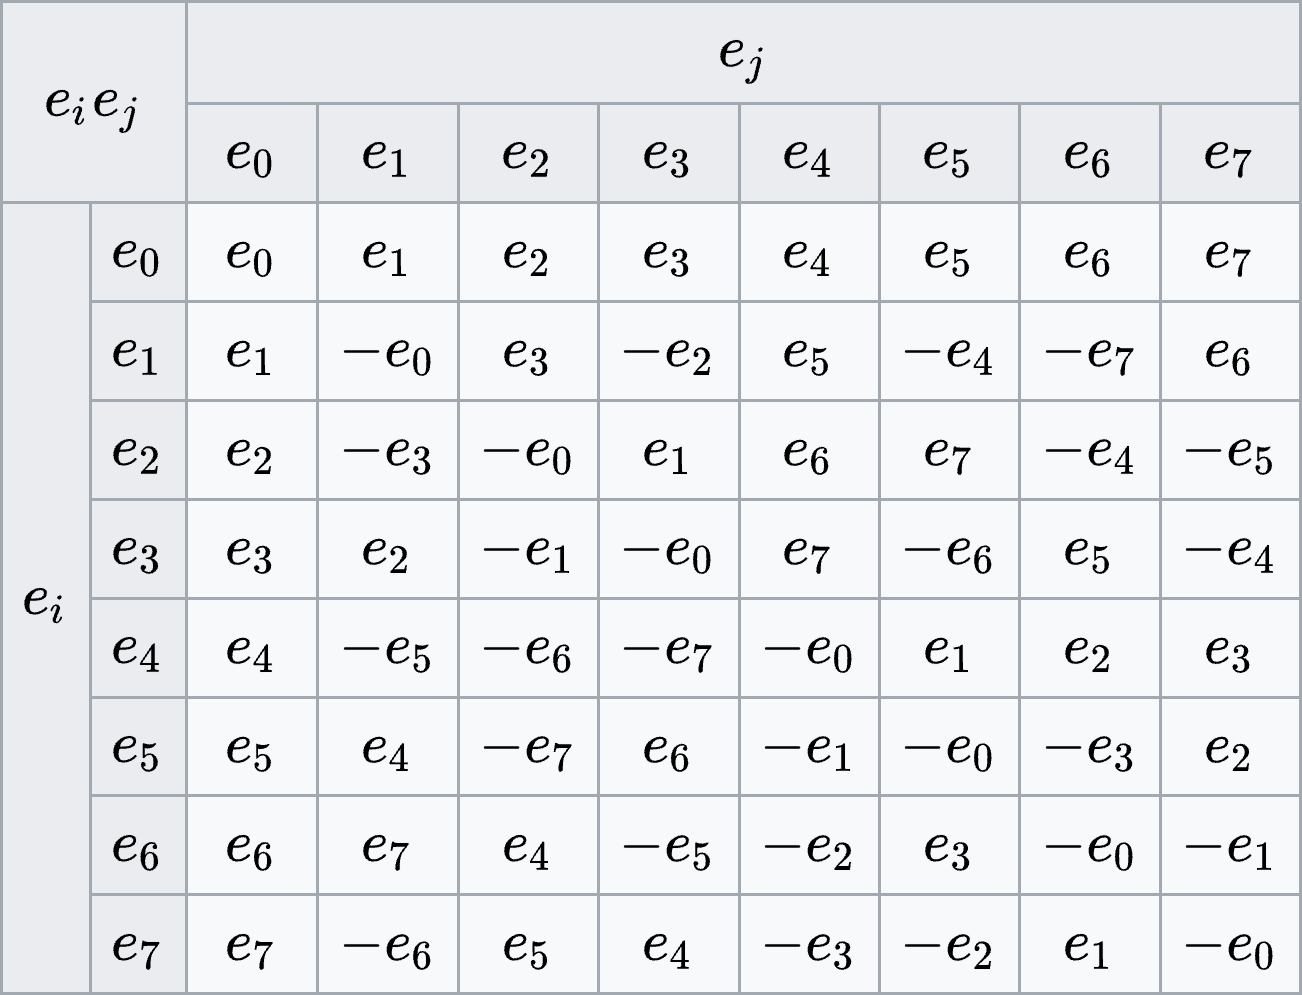
\includegraphics[scale=0.35]{octonion_table.png}
		\caption{The octonion multiplication table with $e_0 = 1$ and the imaginary units $e_1,\dots,e_7$. Screenshot from Wikipedia to avoid formatting a table in \LaTeX{}.}
	\end{figure}
\end{frame}

\begin{frame}
	\frametitle{Relevant quote on octonions}

	\emph{God had no hand in the creation of this abhorrence. The fact that this [number system] exists proves that God is either impotent to alter His universe or ignorant to the horrors taking place in His kingdom. [The octonions are] more than [a number system]. It is a physical declaration of mankind's contempt for the natural order. It is hubris manifest.}
	
	\medskip

	---\texttt{r/copypasta}
\end{frame}

\begin{frame}
	\frametitle{The seven-dimensional cross product}
	\begin{itemize}
		\ii Related to the octonions the same way the three-dimensional cross product is related to the quaternions.
		\ii There are $480$ ways to define the seven-dimensional cross product, compared to only $2$ with the three-dimensional cross product.
		\ii Similarly to the three-dimensional case, $\abs{a \times b} = \abs a\abs b\sin\theta$, where $\theta$ is the angle between $a$ and $b$, $a,b \perp a \times b$, and $a \times b = -b \times a$.
		\ii The cross product \emph{only exists} in three and seven dimensions.
	\end{itemize}
\end{frame}

\end{document}